%-----------------------------------------------%
%             filename: skeleton.tex
%-----------------------------------------------%
\documentclass[aps,twocolumn]{revtex4}
\usepackage{graphicx}
\usepackage{ifpdf}
\ifpdf
	\usepackage[backref]{hyperref}
	%\usepackage[backref,pageanchor=true,plainpages=false, pdfpagelabels,bookmarks,bookmarksnumbered]	{hyperref}
\else
\fi

\usepackage{crs}

% see http://goo.gl/5Fo27
\newtoggle{thmsty}
\toggletrue{thmsty}
%\togglefalse{thmsty}

\begin{document} 

\title{\bf Intrinsic information representation in biological systems}

\author{Cameron Ray Smith$^{1}$, Aviv Bergman$^{1,2,3}$}

\affiliation{$^1$Department of Systems and Computational Biology,\\ $^2$Dominick P. Purpura Department of Neuroscience, \\ $^3$Department of Pathology, Albert Einstein College of Medicine, 1301 Morris Park Ave, Bronx, NY 10461, USA}

\date{\today}
\begin{abstract}
One of the most important aspects of advancing theory and understanding in biology is the development of a constructed language that can be explicitly and precisely defined and supports communication among scientists, between scientists and computers, and even within individual scientists themselves. Such a language should itself be evolvable and support flexible abstractions that enable the unification and compression of redundant information. It would be useful for such a language to be formally specified prior to or in concert with the development of a computational implementation that may support complementary organization of semi-autonomously linked and computable data. We propose the adaptation of a language originally developed in a mathematical context that apparently meets these criteria. We argue for the particular choice we suggest, not from a mathematical perspective but, by providing an example of the way in which this language enables precise qualitative reasoning and flexible methods of abstraction with respect to integrating biological information in a manner that would, ideally, be analogous to the way in which information is integrated by biological systems themselves. Enabling lossless compression and representation of synthetic knowledge about biological systems, in addition to raw biological data, is necessary for understanding in the context of limited cognitive and other computational resources.
\end{abstract}

\maketitle

\tableofcontents

\section{Introduction}
The development of a formal language for modeling biological systems was suggested by Joseph Woodger in collaboration with the developmental biologist Conrad Waddington and the logician Alfred Tarski as early as 1937 \cite{Woodger1937,Woodger1951,Woodger1952,Woodger1952a}. At that time it was perhaps difficult to understand how such a language could be put to use. Today we have tools that could enable the use of such a language: namely 1) computational machines to automate the details of routine transformations within the language and 2) large, accessible, growing repositories of biological data. Though we have access to necessary infrastructure, we lack such a language suggested by Woodger and others throughout the course of the 20th century as we have continued to rely on natural language heuristics to communicate and reason about biological systems.

Category theory \cite{Lane1985,Lane1998,MacLane1992,Lawvere1997,Lawvere2003,Awodey2006} is a language that has been suggested since Woodger to provide a framework for representing and reasoning about biological systems \cite{GOGUEN1979,Ehresmann2007,Louie2009}. What is immediately useful about this language from the perspective of biology is that it presents as primitive the notion of transformation or interaction between objects. In fact, from this point of view, a defining characteristic of any entity (e.g. a protein, cell, organism, or population) is structural: the set of relationships between it and other entities under consideration. Intrinsic properties are taken into account implicitly in this framework since the possible set of relationships between any object and any other is constrained by the nature of its intrinsic properties. 

What is less obvious at first meeting is the way in which category theory, especially with regard to its interface with logic and geometry \cite{MacLane1992,Jacobs1998}, enables the precise definition of what might be viewed as a framework for explaining the nature and development of so-called \emph{emergent properties} of systems of interacting processes. This expression is general enough that it can be equally well applied to the consideration of relationships between any levels of biological organization and may be generalizable to arbitrary physical contexts. This unity deriving from the judicious definition of underlying categorical concepts along the way is precisely the type of abstraction that we argue is necessary to enable compression without loss of biological information and thus synthesis of existing biological knowledge.

Here we define the concepts from category theory necessary to understand the way in which interacting objects at one level of organization (e.g. molecules) can produce phenomena that would themselves be identifiable as derived objects (e.g. cells) that justify the very conceptualization of a \emph{level of organization} in the first instance. Here we focus exclusively on defining the boundary conditions relating levels (e.g. molecules and cells or cells and multicellular organisms) of organization, which are necessary to understand in the course of defining a dynamical system that could model the \emph{evolution} of such. What results is a refinement of the concept of the levels of organization that are ubiquitously employed in biology and examples of which are used so far only heuristically as guides to pre-existing intuition. Understanding how to integrate information regarding biological processes across such levels of organization is fundamental to the understanding of complex phenotypes and the associated set of contingencies necessary to account for in methods that may be targeted at controlling or otherwise manipulating them.

[ Note that biological systems are concretely represented as graphs of some kind and all the letters representing categories can be specialized to categories of graphs of some kind ]

\section{Biological information}
\subsection{Biological system-environment duality}
Distinction between biological systems or some components thereof and the environments within which they are embedded is implied in models of such systems. This distinction is useful in many contexts, but the boundary between a biological system and its environment is dependent upon the level of resolution of the \emph{model and modeler} independent of its relationship to properties of the biological system itself \cite{Fontana1996}. In this light, it is desirable to develop a model of biological systems that supports variation of this boundary without requiring any reconfiguration of the model. Constructing a framework for such models requires the determination, unification, and incorporation of abstract features of biological systems that are invariant across levels of organization from molecules to cells, organisms, populations, communities, ecosystems and more fine-grained levels of resolution that likely lie between these broadly and imprecisely defined perspectives one can take with regard to representing biological systems.


\subsection{Transformation of biological information at system-environment boundaries}
The use of categorical adjunctions to model information representation in biological systems has been suggested \cite{GOGUEN1979,Ellerman2007,Ellerman2008}, but these efforts have yet to be incorporated into more detailed theories. We begin here by developing the prerequisite definitions to explain why the transformation of biological information is naturally represented as a pair of adjoint functors in the context of category theory.

\iftoggle{thmsty}{
\begin{definition}
\label{definition-category}
}{}
A {\it category} $\mathcal{C}$ is:
\begin{enumerate}
\item A set of objects $\Ob(\mathcal{C})$.
\item For each pair $x, y \in \Ob(\mathcal{C})$ a set of morphisms
$\Mor_\mathcal{C}(x, y)$.
\item For each triple $x, y, z\in \Ob(\mathcal{C})$ a composition
map $ \Mor_\mathcal{C}(y, z) \times \Mor_\mathcal{C}(x, y)
\to \Mor_\mathcal{C}(x, z) $, denoted $(\phi, \psi) \mapsto
\phi \circ \psi$.
\end{enumerate}
Such that these constraints are satisfied:
\begin{enumerate}
\item For every element $x\in \Ob(\mathcal{C})$ there exists a
morphism $\text{id}_x\in \Mor_\mathcal{C}(x, x)$ such that
$\text{id}_x \circ \phi = \phi$ and $\psi \circ \text{id}_x = \psi $.
\item Composition is associative, i.e., $(\phi \circ \psi) \circ \chi =
\phi \circ ( \psi \circ \chi)$.
\end{enumerate}
\iftoggle{thmsty}{
\end{definition}
}

\iftoggle{thmsty}{
\begin{definition}
\label{definition-functor}
}{}
A {\it functor} $F : \mathcal{A} \to \mathcal{B}$
between two categories $\mathcal{A}, \mathcal{B}$ is:
\begin{enumerate}
\item A map $F : \Ob(\mathcal{A}) \to \Ob(\mathcal{B})$.
\item For every $x, y \in \Ob(\mathcal{A})$ a map
$F : \Mor_\mathcal{A}(x, y) \to \Mor_\mathcal{B}(F(x), F(y))$,
denoted $\phi \mapsto F(\phi)$.
\end{enumerate}
These data should be compatible with composition and identity morphisms
in the following manner: $F(\phi \circ \psi) =
F(\phi) \circ F(\psi)$ for a composable pair $(\phi, \psi)$ of
morphisms of $\mathcal{A}$ and $F(\text{id}_x) = \text{id}_{F(x)}$.
\iftoggle{thmsty}{
\end{definition}
}

\iftoggle{thmsty}{
\begin{definition}
\label{definition-transformation-functors}
}{}
Let $F, G : \mathcal{A} \to \mathcal{B}$ be functors.
A {\it natural transformation}, or a {\it morphism of functors}
$t : F \to G$, is a collection $\{t_x\}_{x\in \Ob(\mathcal{A})}$
such that
\begin{enumerate}
\item $t_x : F(x) \to G(x)$ is a morphism in the category $\mathcal{B}$, and
\item for every morphism $\phi : x \to y$ of $\mathcal{A}$ the following
diagram is commutative
$$
\xymatrix{
F(x) \ar[r]^{t_x} \ar[d]_{F(\phi)} & G(x) \ar[d]^{G(\phi)} \\
F(y) \ar[r]^{t_y} & G(y) }
$$
\end{enumerate}
\iftoggle{thmsty}{
\end{definition}
}

We can define a category having functors as objects and natural transformations as morphisms, which is called a functor category, by recognizing that every functor $F$ comes with the {\it identity} transformation $\text{id}_F : F \to F$. In addition, given a morphism of
functors $t : F \to G$ and a morphism of functors $s : E \to F$
then the {\it composition} $t \circ s$ is defined by the rule
$$
(t \circ s)_x = t_x \circ s_x : E(x) \to G(x)
$$
for $x \in \Ob(\mathcal{A})$.
This is a morphism of functors
from $E$ to $G$.
Thus, given categories
$\mathcal{A}$ and $\mathcal{B}$ we obtain the category of functors between $\mathcal{A}$ and
$\mathcal{B}$.

\iftoggle{thmsty}{
\begin{definition}
\label{definition-equivalence-categories}
}{}
An {\it equivalence of categories}
$F : \mathcal{A} \to \mathcal{B}$ is a functor such that there
exists a functor $G : \mathcal{B} \to \mathcal{A}$ such that
the compositions $F \circ G$ and $G \circ F$ are isomorphic to the
identity functors $\text{id}_\mathcal{B}$,
respectively $\text{id}_\mathcal{A}$.
In this case we say that $G$ is a {\it quasi-inverse} to $F$.
\iftoggle{thmsty}{
\end{definition}
}

\iftoggle{thmsty}{
\begin{definition}
\label{definition-adjoint}
}{}
Let $\mathcal{C}$, $\mathcal{D}$ be categories.
Let $u : \mathcal{C} \to \mathcal{D}$ and
$v : \mathcal{D} \to \mathcal{C}$ be functors.
We say that $u$ is a {\it left adjoint} of $v$ or that
$v$ is a {\it right adjoint} to $u$, written $u \dashv v$, if there are bijections
$$
\phi_{X,Y}:\Mor_\mathcal{D}(u(X), Y)
\simeq
\Mor_\mathcal{C}(X, v(Y))
$$
functorial in $X \in \Ob(\mathcal{C})$, and
$Y \in \Ob(\mathcal{D})$.
\iftoggle{thmsty}{
\end{definition}
}

Morphisms that are associated with each other according to the bijections of an adjunction are called {\it adjoint transposes} of one another. If $g:u(X) \rightarrow Y$, $g \in \Mor(\cD)$ then $g^*: X \rightarrow v(Y)$, $g^* \in \Mor(\cC)$ is given by $\phi_{X,Y}(g) = g^*$. Similarly for $f: X \rightarrow v(Y)$, $f \in \Mor(\cC)$ with $f^*:u(X) \rightarrow Y$, $f^* \in \Mor(\cD)$ is given by $\phi_{X,Y}^{-1}(f) = f^*$. We see then that $g^* = f$ and $f^* = g$.

\iftoggle{thmsty}{
\begin{definition}
\label{definition-opposite}
}{}
Given a category $\mathcal{C}$ the {\it opposite category}
$\mathcal{C}^{opp}$ is the category with the same objects
as $\mathcal{C}$ but all morphisms reversed.
\iftoggle{thmsty}{
\end{definition}
}

\iftoggle{thmsty}{
\begin{definition}
\label{definition-contravariant}
}{}
Let $\mathcal{C}$, $\mathcal{S}$ be categories.
A {\it contravariant} functor $F$
from $\mathcal{C}$ to $\mathcal{S}$
is a functor $\mathcal{C}^{opp}\to \mathcal{S}$.
\iftoggle{thmsty}{
\end{definition}
}

\iftoggle{thmsty}{
\begin{definition}
\label{definition-presheaf}
}{}
Let $\mathcal{C}$ be a category.
\begin{enumerate}
\item A {\it presheaf of sets on $\mathcal{C}$}
or simply a {\it presheaf} is a contravariant functor
$F$ from $\mathcal{C}$ to $\textit{Sets}$. When $F$ is a covariant functor $F : \mathcal{C}^{opp} \rightarrow \textit{Sets}$.
\item The category of presheaves is denoted $\textit{PSh}(\mathcal{C})$.
\end{enumerate}
\iftoggle{thmsty}{
\end{definition}
}

\iftoggle{thmsty}{
\begin{definition}
\label{definition-products}
}{}

Let $x, y\in \Ob(\mathcal{C})$,
A {\it product} of $x$ and $y$ is
an object $x \times y \in \Ob(\mathcal{C})$
together with morphisms
$p\in \Mor_{\mathcal C}(x \times y, x)$ and
$q\in\Mor_{\mathcal C}(x \times y, y)$ such
that the following universal property holds: for
any $w\in \Ob(\mathcal{C})$ and morphisms
$\alpha \in \Mor_{\mathcal C}(w, x)$ and
$\beta \in \Mor_\mathcal{C}(w, y)$
there is a unique
$\gamma\in \Mor_{\mathcal C}(w, x \times y)$ making
the diagram
$$
\xymatrix{
w \ar[rrrd]^\beta \ar@{-->}[rrd]_\gamma \ar[rrdd]_\alpha & & \\
& & x \times y \ar[d]_p \ar[r]_q & z \\
& & x &
}
$$
commute.
\iftoggle{thmsty}{
\end{definition}
}

\iftoggle{thmsty}{
\begin{definition}
\label{definition-has-products-of-pairs}
}{}
We say the category $\mathcal{C}$ {\it has products of pairs
of objects} if a product $x \times y$
exists for any $x, y \in \Ob(\mathcal{C})$.
\iftoggle{thmsty}{
\end{definition}
}

\iftoggle{thmsty}{
\begin{definition}
\label{definition-coproducts}
}{}
Let $x, y \in \Ob(\mathcal{C})$,
A {\it coproduct}, or {\it amalgamated sum} of $x$ and $y$ is
an object $x \amalg y \in \Ob(\mathcal{C})$
together with morphisms
$i \in \Mor_{\mathcal C}(x, x \amalg y)$ and
$j \in \Mor_{\mathcal C}(y, x \amalg y)$ such
that the following universal property holds: for
any $w \in \Ob(\mathcal{C})$ and morphisms
$\alpha \in \Mor_{\mathcal C}(x, w)$ and
$\beta \in \Mor_\mathcal{C}(y, w)$
there is a unique
$\gamma \in \Mor_{\mathcal C}(x \amalg y, w)$ making
the diagram
$$
\xymatrix{
& y \ar[d]^j \ar[rrdd]^\beta \\
x \ar[r]^i \ar[rrrd]_\alpha & x \amalg y \ar@{-->}[rrd]^\gamma \\
& & & w
}
$$
commute.
\iftoggle{thmsty}{
\end{definition}
}

\iftoggle{thmsty}{
\begin{definition}
\label{definition-has-coproducts-of-pairs}
}{}
We say the category $\mathcal{C}$ {\it has coproducts of pairs
of objects} if a coproduct $x \amalg y$
exists for any $x, y \in \Ob(\mathcal{C})$.
\iftoggle{thmsty}{
\end{definition}
}

\iftoggle{thmsty}{
\begin{definition}
\label{definition-product-category}
}{}
Let $\mathcal{A}$, $\mathcal{B}$ be categories.
The {\it product category} is the category
$\mathcal{A} \times \mathcal{B}$ with
objects
$\Ob(\mathcal{A} \times \mathcal{B}) =
\Ob(\mathcal{A}) \times \Ob(\mathcal{B})$
and
$$
\Mor_{\mathcal{A} \times \mathcal{B}}((x, y), (x', y'))
:=
\Mor_\mathcal{A}(x, x')\times
\Mor_\mathcal{B}(y, y').
$$
Composition of morphisms is defined according to components.
\iftoggle{thmsty}{
\end{definition}
}

\iftoggle{thmsty}{
\begin{definition}
\label{definition-bifunctor}
}{}
Given categories $\mathcal{C}_1$, $\mathcal{C}_2$, and $\mathcal{D}$. A {\it bifunctor} or binary functor or 2-ary functor or functor of two variables, $F$, is a functor whose domain is the product of two categories $F: \mathcal{C}_1 \times \mathcal{C}_2 \rightarrow \mathcal{D}$.
\iftoggle{thmsty}{
\end{definition}
}

\iftoggle{thmsty}{
\begin{definition}
\label{definition-hom-functor}
}{}
The {\it hom-functor} is a bifunctor defined on the product of a category $\mathcal{C}$ with its self-dual category $\mathcal{C}^{opp}$, which takes values in the category $\textit{Sets}$. Thus for a category $C$ its hom-functor is 
$$
hom(-,-): \mathcal{C}^{opp} \times \mathcal{C} \rightarrow \textit{Sets}.
$$
The hom-functor maps
\begin{enumerate}
\item objects $(c,c') \in \mathcal{C}^{opp} \times \mathcal{C}$ to the hom-set $\Mor_{\mathcal{C}} (c,c')$, which is the set of morphisms in $\mathcal{C}$ with domain $c$ and codomain $c'$.
\item morphisms 
$$
(f,g):(c,c') \rightarrow (d,d') \in \Mor(\mathcal{C}^{opp} \times \mathcal{C}),
$$
where $f:d \rightarrow c \in \Mor(\mathcal{C})$ and $g:c' \rightarrow d' \in \Mor(\mathcal{C})$, to the set function
\begin{eqnarray*}
\Mor_{\mathcal{C}}(c,c') &\rightarrow& \Mor_{\mathcal{C}}(d,d')\\
(c \rightarrow c') &\mapsto& (d \rightarrow c \rightarrow c' \rightarrow d')
\end{eqnarray*}
\end{enumerate}
\iftoggle{thmsty}{
\end{definition}
}

\iftoggle{thmsty}{
\begin{definition}
\label{definition-representable-functor}
}{}
For a hom-functor $hom(-,-): \mathcal{C}^{opp} \times \mathcal{C} \rightarrow \textit{Sets}$ for $c \in \Ob(\mathcal{C})$ a covariant and contravariant functor can be derived by specializing the hom-functor to morphisms out of or into the object $c$ as
\begin{eqnarray*}
h^c \equiv hom(-,c) &:& \mathcal{C}^{opp} \rightarrow \textit{Sets}\\
h_c \equiv hom(c,-) &:& \mathcal{C} \rightarrow \textit{Sets}.
\end{eqnarray*}
Functors that are isomorphic to $h^c$ or $h_c$ are referred to as {\it corepresentable or representable functors} respectively and $c$ is their {\it representing object}. Note that $h_c \in \Ob(\textit{PSh}(\mathcal{C}))$.
\iftoggle{thmsty}{
\end{definition}
}

The preceding definitions are standard category theoretic constructions. Ellerman has proposed an interpretation of adjoint functors, that demonstrates their relevance to the concept of information encoding and decoding (or sending and receiving) in the context of biological systems \cite{Ellerman2005}.

\iftoggle{thmsty}{
\begin{definition}
\label{definition-birepresentable}
}{}
A bifunctor $bif (-,-): \cC^{opp} \times \cD \rightarrow \textit{Sets}$ is said to be {\it birepresentable} if there exists a pair of functors $F:\cC^{opp} \rightleftarrows \cD:G$ where $c \in \Ob(\cC^{opp})$ and $d \in \Ob(\cD)$ gives
\begin{eqnarray*}
b^{d} \equiv bif(-,d) &:& \mathcal{C}^{opp} \rightarrow \textit{Sets},\\
b_{c} \equiv bif(c,-) &:& \mathcal{D} \rightarrow \textit{Sets}.
\end{eqnarray*}
natural in $c$ and $d$ such that $F \dashv G$. The functors $b^{d}$ and $b_{c}$ are defined on
\begin{enumerate}
\item objects for all $c_i \in \Ob(\cC^{opp})$ and for all $d_i \in \Ob(\cD)$
\begin{eqnarray*}
b^{d} (c_i) &=& \Mor_{\cC^{opp}}(c_i,Gd),\\
b_{c} (d_i) &=& \Mor_{\cD}(Fc,d_i).
\end{eqnarray*}

\item morphisms for all $f_{ij}:c_j \rightarrow c_i \in \Mor(\cC^{opp})$ and for all $g_{ij}:d_i \rightarrow d_j \in \Mor(\cD)$ as
\begin{eqnarray*}
b^{d} (f_{ij}) &:& \Mor_{\cC^{opp}}(c_i,Gd) \rightarrow \Mor_{\cC^{opp}}(c_j,Gd),\\
b_{c} (g_{ij}) &:& \Mor_{\cD}(Fc,d_i) \rightarrow \Mor_{\cD}(Fc,d_j).
\end{eqnarray*}
\end{enumerate}
\iftoggle{thmsty}{
\end{definition}
}

$F \dashv G$ is thus equivalent to the statement $\phi_{-,-}:b_{(-)} \cong b^{(-)}$. In this framework, information encoding/decoding is an asymmetric process that can only be accomplished without loss of information in one direction: objects of $\cD$ can be encoded into objects of $\cC$ and decoded into objects of $\cD$ but, in general, proceeding in the opposite order may result in loss of information. This asymmetry is clarified by consideration of the unit and counit morphisms of the adjunction.

\iftoggle{thmsty}{
\begin{definition}
\label{definition-unit}
}{}
Consider the identity morphism $1_{Fc} \in \Mor_{\cD}(Fc,Fc)$. The adjoint transpose of $1_{Fc}$ is the {\it unit} morphism at $c$
$$
\phi_{c,Fc}(1_{Fc})=1_{Fc}^*=\eta_c: c \rightarrow GFc
$$
where $\eta_c \in \Mor_{\cC^{opp}}(c,GFc)$, which, when taken to hold quantifying over all $c \in \Ob(\cC^{opp})$ (i.e. to be natural in $c$), gives the natural transformation
$$
\eta : 1_{\cC^{opp}} \rightarrow GF
$$
\iftoggle{thmsty}{
\end{definition}
}

\iftoggle{thmsty}{
\begin{definition}
\label{definition-counit}
}{}
Consider the identity morphism $1_{Gd} \in \Mor_{\cC^{opp}}(Gd,Gd)$. The adjoint transpose of $1_{Gd}$ is the {\it counit} morphism at $d$
$$
\phi_{Gd,d}^{-1}(1_{Gd})=1_{Gd}^*=\epsilon_d: FGd \rightarrow d
$$
where $\epsilon_d \in \Mor_{\cD}(d,FGd)$, which, when natural in $d$, gives the natural transformation
$$
\epsilon: FG \rightarrow 1_{\cD}
$$
\iftoggle{thmsty}{
\end{definition}
}

The composite encoding inspection functor 
$$
b_{(-)} \circ G(-): \cD \rightarrow \cC^{opp} \rightarrow \textit{Sets}
$$
that specifies a set of morphisms in $\cD$ from the perspective of $\cC^{opp}$ is represented by the pair $(F,\eta)$. Likewise, the composite decoding inspection functor 
$$
b^{(-)} \circ F(-): \cC^{opp} \rightarrow \cD \rightarrow \textit{Sets}
$$
that specifies a set of morphisms in $\cC^{opp}$ from the perspective of $\cD$ is represented by the pair $(G,\epsilon)$.

\subsection{Intrinsic measurement processes of biological systems}

\subsection{Topological features of biological information}

\subsection{Variable filtration of biological information}

\subsection{Deconstructing and synthesizing biological information}

\subsection{Enabling conditions of hierarchical transformations}


\section{Biological evolution}
\subsection{Niche construction and multilevel selection}
Selection is part of any evolutionary process. Niche construction, which is complementary to selection, has been introduced more recently \cite{Odling-Smee2003,Krakauer2009}. An organism experiences a situation similar to that represented in diagram \ref{eq:intrep}. 

\begin{equation} \label{eq:intrep}
\begin{tikzcd}[column sep=huge,row sep=huge,baseline=(current bounding box.center)]
\mathcal{D}
  \arrow[loop left]{}[name=fg]{F \circ G}
  \rar[start anchor=30, end anchor=151]{G}
  \arrow{d}[swap,name=h]{H} & 
\mathcal{J}\lar[start anchor=196, end anchor=-14]{F} \\
\mathcal{C}
\arrow[shorten >=3pt,Rightarrow,to path={(fg.290) to[out=-90,in=180] node[xshift=-3.5mm] {$\eta$} (h)}]{}
\end{tikzcd}
\end{equation} 

The molecular interaction network that underlies an arbitrary type of organism is represented by a category $\mathcal{D}$ and the environment is represented by a category $\mathcal{C}$. Due to the dependence of selection on the environment, those organisms capable of survival are those that most closely approximate a natural transformation $\eta:F \circ G \Rightarrow H$. Why might this be the case?

To answer this question requires consideration of the necessity of the category $\mathcal{J}$ in this conceptual framework. From the perspective of any organism, we can roughly think of $\mathcal{D}$ as ''internal'' and $\mathcal{C}$ as ''external'' in a sense that can be likened but not yet clearly identified with ''known'' and ''unknown'' respectively. The selection process can be thought of as requiring the organism to establish a representation of properties of $\mathcal{C}$ so as to enable its existence to remain complementary, and thus stable, relative to its environment. The molecular network underlying the various biochemical functions of the organism has no direct access to the processes that determine the causal structure of the environment. In this case we consider the organism to have direct access only to the structure contained in $\mathcal{D}$, but nevertheless being implicitly assigned, as a result of its relationship to the environment, the seemingly impossible task of establishing the structure of $\mathcal{C}$. If $\mathcal{C}$ were internalized by the organism then relationships between $\mathcal{D}$ and $\mathcal{C}$ that preserve structure, specifically the functors labelled $H:\mathcal{D} \rightarrow \mathcal{C}$, could also be directly internalized. Since $\mathcal{C}$ is external to $\mathcal{D}$, the organism must find another way of determining the relationship between its internal structure and that which is external, even if local.

One way to address this apparently paradoxical situation is to consider the relationship between endofunctors on $\mathcal{D}$ and those like $H$. In the case of \ref{eq:intrep}, $\mathcal{J}$ is considered to be a subcategory of $\mathcal{D}$ that contains all the domains (in the sense of complete partial orders) of $\mathcal{D}$. This scenario allows functors $F:\mathcal{J} \rightarrow \mathcal{D}$ to index diagrams in $\mathcal{D}$.

See \cite{Okasha2006} for information on multilevel selection.

\subsection{The structure of molecular networks}
\subsubsection{Endo-genetics, genetics, epi-genetics, and $n$-epi-genetics}
\subsection{Hierarchical organization and evolution}
See \cite{Gould1994}, \cite{Arnold1982}.

\section{Hierarchy in logic}

\subsection{Russell's paradox}
A theorem due to Cantor states that given a set $X$ and a map of sets $f$ it is impossible to find a mapping $$ f: X \rightarrow 2^X $$ where $2^X$ represents the set of all subsets of $X$ also referred to as the powerset of $X$.

\subsection{A type theoretic resolution}

\subsection{Categorical type theory}
See \cite{Crole1994a}.

\section{Information representation}

\subsection{Information theory}
See \cite{Ellerman2008} and \cite{Cover2006}.

\subsection{Domain theory}
See \cite{Abramsky}, \cite{Abramsky1995}.

\subsection{Game semantics}
See \cite{Mellies2009}

\section*{Acknowledgements} 

CRS was supported by . 
AB was supported by .

%-----------------------------------------------%
%                   appendix
%-----------------------------------------------%
\appendix
\section{Category theory for tourists}
%\begin{figure}
%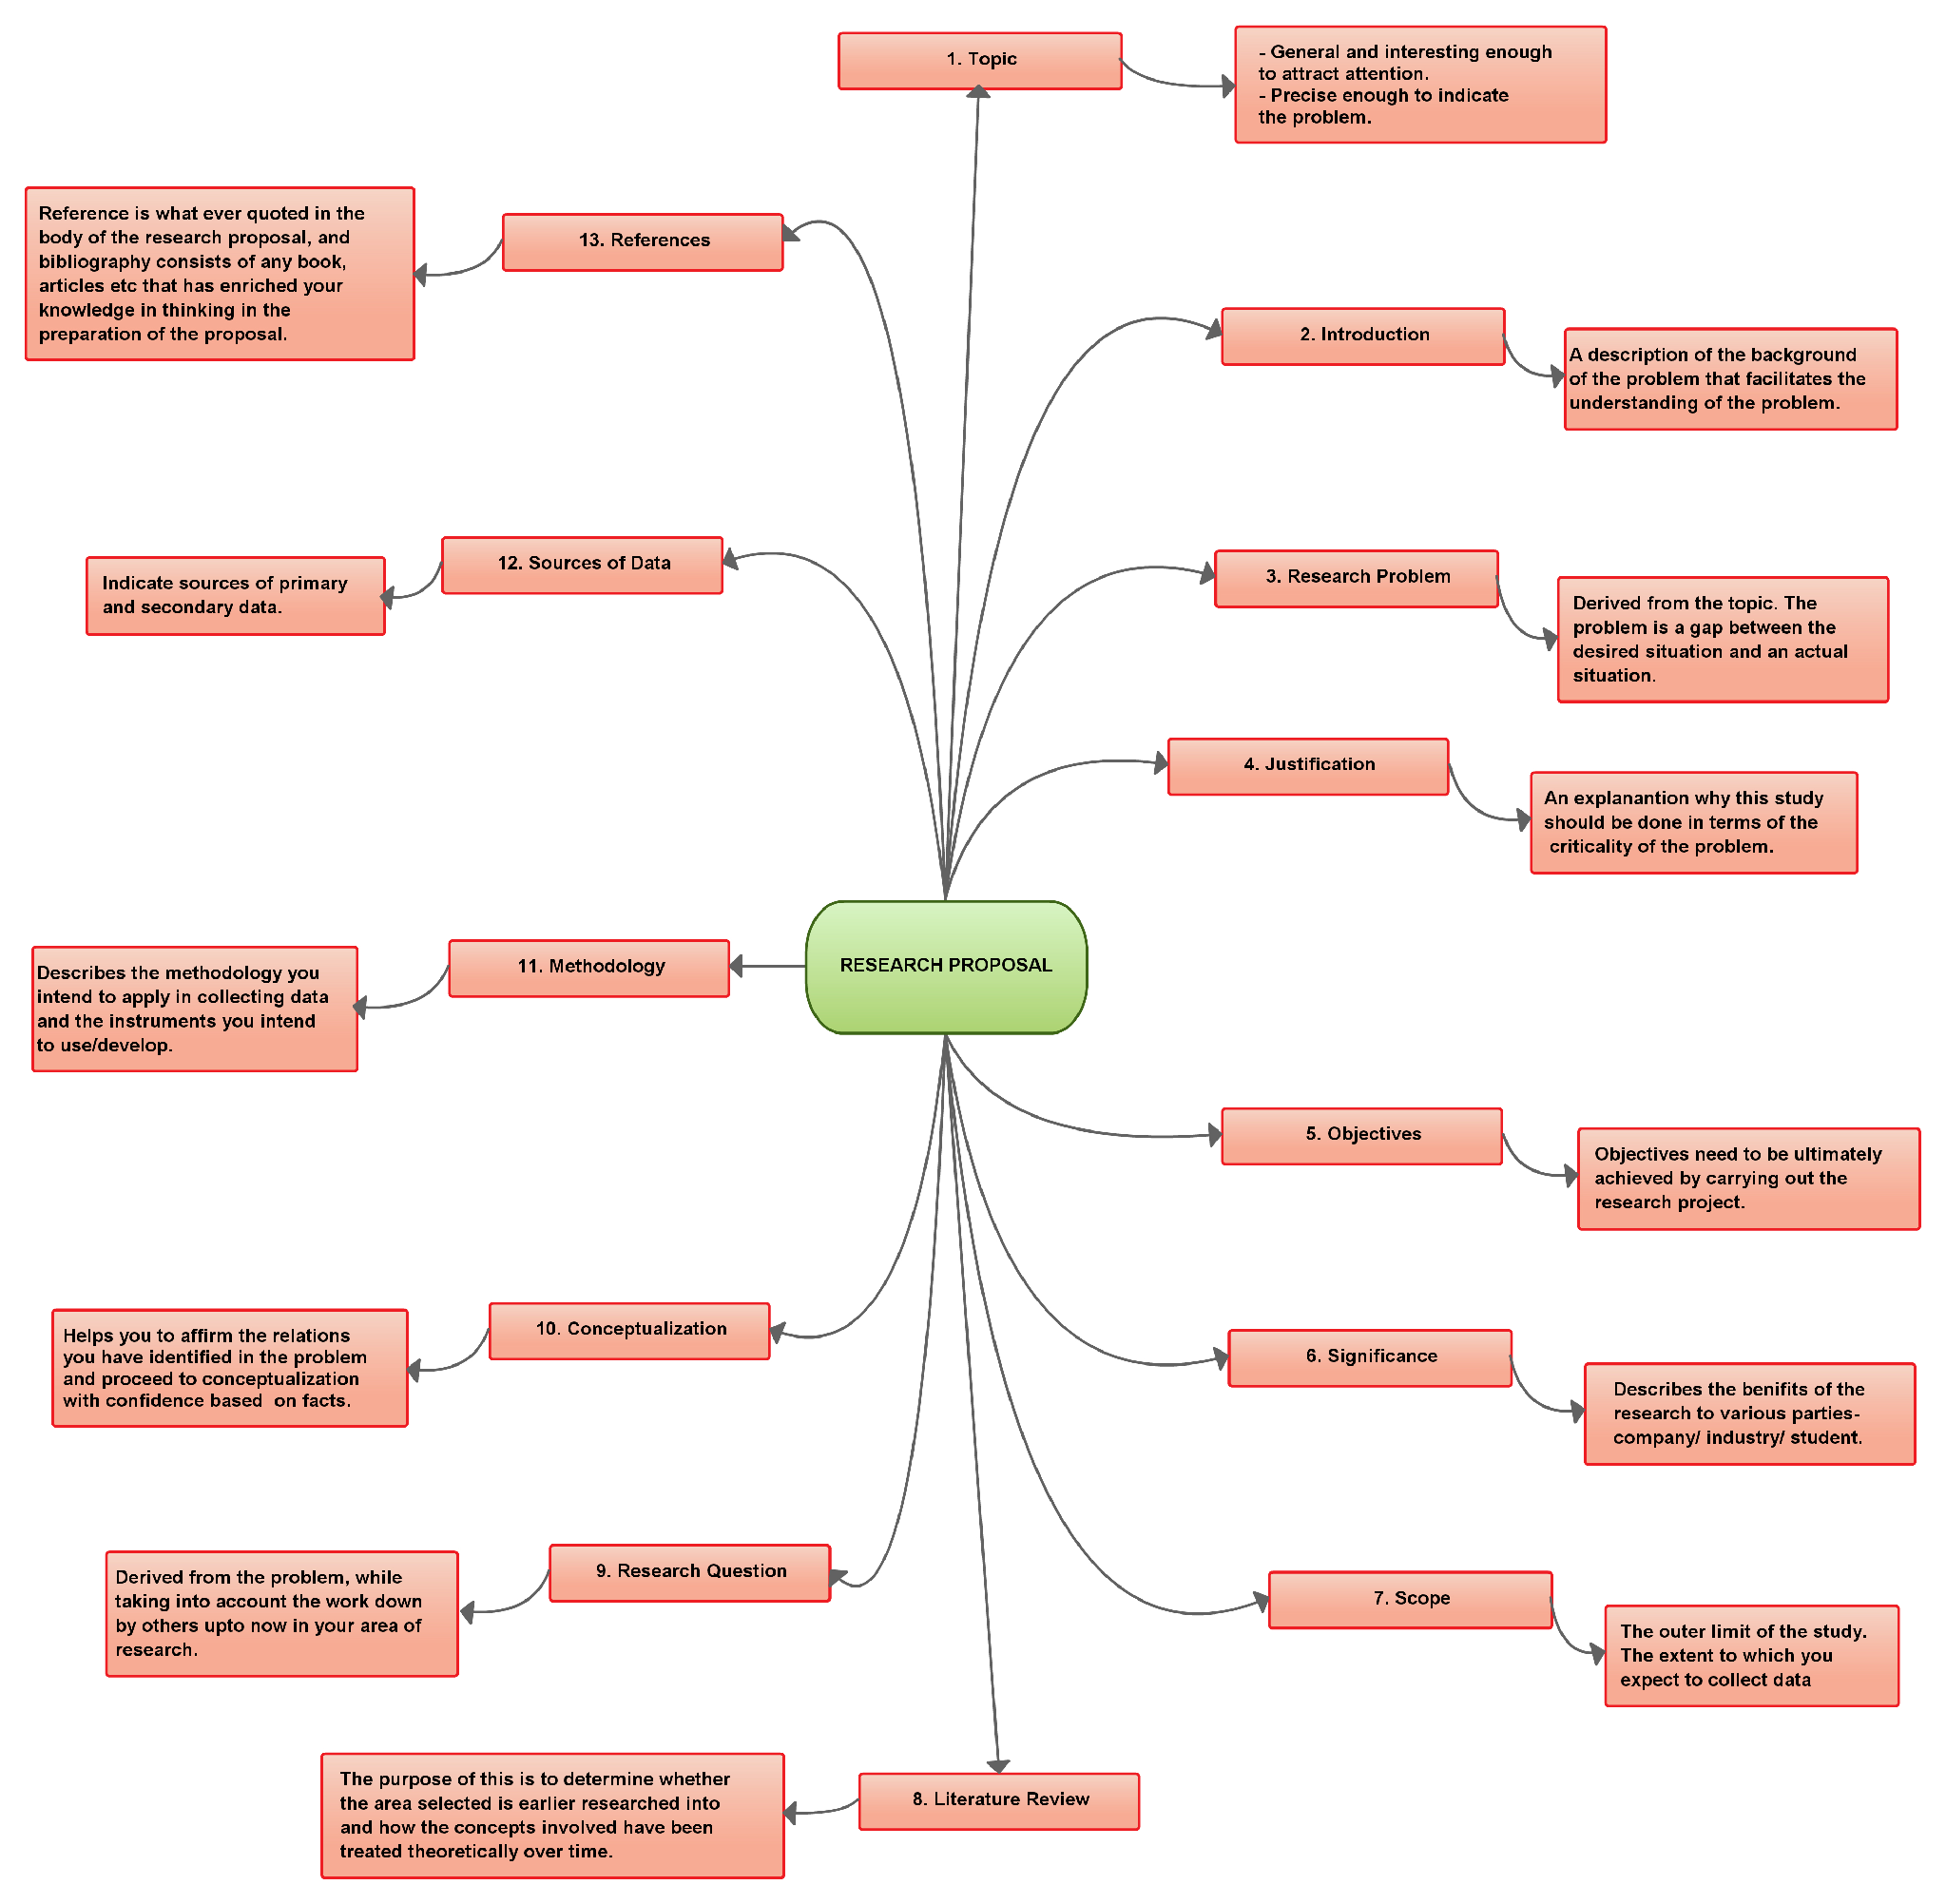
\includegraphics[scale=0.2]{fig/createlytest1.pdf}
%\caption{This is a $\implies$ creately.com diagram}
%\end{figure}
%
%\begin{center}
%\asyinclude{fig/comdiag.asy}
%\end{center}
%
%\begin{equation}\label{eq:star}
%\xymatrix{
%{\mathcal V}  \ar[r]^{S \quad\quad } \ar[d]_{\pi}
%&  \mathsf{DynSys} \ar[d]^{U}  \\
% \op{(\et{\Graph})}  \ar[r]^{\quad\mathbb{P} }
%&  \mathsf{Man} }
%\end{equation}
%
%Two related questions \cite{Gould1994} define a fundamental role for statistical
%physics in systems biology: (1). How do biomolecular systems achieve
%reliable ``device-level'' behavior when they consist of highly
%
%\begin{equation*}
%\xy
%(-18, 10)*+{\PP\lv T} ="1"; 
%(18, 10)*+{\PP\rt T} ="2";
%(-18,-10)*+{\PP\lv T'}="3";
%(18,-10)*+{\PP \rt T'}="4";
%{\ar@{->}^X "1";"2"};
%{\ar@{->}^{\PP(\sigma|_{\lv T})} "3";"1"};
%{\ar@{=}_{\PP(\sigma|_{\rt T}) = id } "4";"2"};
%{\ar@{-->}_{\Ctrl(\sigma)X} "3";"4"};
%\endxy
%\end{equation*}
%
%\begin{center}
%\begin{tikzpicture}[shorten >=1pt,->]
%  \tikzstyle{vertex}=[circle,fill=black!25,minimum size=17pt,inner sep=0pt]
%
%  \foreach \name/\x in {s/1, 2/2, 3/3, 4/4, 15/11, 
%                        16/12, 17/13, 18/14, 19/15, t/16}
%    \node[vertex] (G-\name) at (\x,0) {$\name$};
%
%  \foreach \name/\angle/\text in {P-1/234/5, P-2/162/6, 
%                                  P-3/90/7, P-4/18/8, P-5/-54/9}
%    \node[vertex,xshift=6cm,yshift=.5cm] (\name) at (\angle:1cm) {$\text$};
%
%  \foreach \name/\angle/\text in {Q-1/234/10, Q-2/162/11, 
%                                  Q-3/90/12, Q-4/18/13, Q-5/-54/14}
%    \node[vertex,xshift=9cm,yshift=.5cm] (\name) at (\angle:1cm) {$\text$};
%
%  \foreach \from/\to in {s/2,2/3,3/4,3/4,15/16,16/17,17/18,18/19,19/t}
%    \draw (G-\from) -- (G-\to);
%
%  \foreach \from/\to in {1/2,2/3,3/4,4/5,5/1,1/3,2/4,3/5,4/1,5/2}
%    { \draw (P-\from) -- (P-\to); \draw (Q-\from) -- (Q-\to); }
%
%  \draw (G-3) .. controls +(-30:2cm) and +(-150:1cm) .. (Q-1);
%  \draw (Q-5) -- (G-15);
%\end{tikzpicture}
%\end{center}
%
%
%\usetikzlibrary{matrix,arrows}
%\begin{equation}
%\begin{tikzpicture}[description/.style={fill=white,inner sep=2pt}, baseline=(current bounding box.center)]
%	\matrix (m) [matrix of math nodes, row sep=3em,
%	column sep=2.5em, text height=1.5ex, text depth=0.25ex]
%	{ A & & B \\
%	& C & \\ };
%	\path[->,font=\scriptsize]
%	(m-1-1) edge node[auto] {$ \varphi $} (m-1-3)
%	edge node[description] {$ \Psi $} (m-2-2)
%	(m-1-3) edge node[auto] {$ \Phi $} (m-2-2);
%\end{tikzpicture}
%\end{equation}

%------bibliography---%
\bibliographystyle{unsrt} 
%\bibliography{ref/HO}
\bibliography{bib/books,bib/papers}
%\bibliography{library}
%---------------------%

\end{document}